\chapter{Conceitos Básicos}
Nesta seção, iremos explorar alguns fundamentos básicos para compreender, passo a passo, como será conduzida a metodologia proposta. Primeiramente será introduzido uma abstração matemática muito utilizada na computação, o Grafo, que têm como serventia facilitar a visualização de como é composto uma estrutura de um neurônio artificial. Feito isso, descrevemos brevemente sobre classificação de dados e também sobre duas técnicas de categorização, as Redes Neurais Artificiais (RNA) e o K-vizinhos mais próximos (do inglês: \textit{K-Nearest Neighbors} - KNN). Por fim, é apresentado uma breve introdução ao Processamento de Linguagem Natural (PLN), uma sub-área da da Inteligência Artificial (IA).

\section{Grafos}
Muitas situações no mundo real podem ser descritas com o uso de um diagrama, composto por um conjunto de pontos e arestas, onde as arestas unem pares desses pontos. Por exemplo, os pontos podem representar cidades em um mapa, e as arestas representariam as estradas que ligam duas cidades. O conceito de grafo parte de uma abstração matemática para caracterizar situações com essas características \citep{Bondy1976}.

Matematicamente um grafo $G$ é uma tripla ($V$, $E$, $\psi$), consistido por um conjunto não vazio de vértices $V$, um conjunto de arestas $E$ e uma função de incidência $\psi$ que caracteriza quais vértices possuem uma relação (através de uma aresta) com outros vértices. Por exemplo, seja $G = (V, E, \psi)$ um grafo (Figura \ref{fig:graphExample1}), tal que $V = \{0, 1, 2, 3, 4, 5\}$, $E = \{a, b, c, d, e, f, g, i\}$ e $\psi$ a função incidência representada na Tabela \ref{tab:graphExample1}.

\begin{table}[ht!]
\caption{Função incidência $\psi$ de $G$}
\label{tab:graphExample1}
\centering
\begin{tabular}{| c | c |}
\hline
    $\psi_a = 1,2$\\ 
    $\psi_b = 2,0$\\ 
    $\psi_c = 1,0$\\ 
    $\psi_d = 4,3$\\
    $\psi_e = 4,5$\\
    $\psi_f = 5,3$\\
    $\psi_g = 2,5$\\
    $\psi_h = 1,4$\\
    $\psi_i = 4,3$\\
\hline
\end{tabular}
{\fontsize{11pt}{\baselineskip}\selectfont
\\Fonte: Elaborado pelo autor.
}
\end{table}

Segundo \cite{Bondy1976}, os grafos possuem esse nome porque eles possuem uma representação gráfica, e são essas representações que facilitam o entendimento de suas propriedades.

\begin{figure}[ht!]
\caption{Diagrama do Grafo $G$}
\label{fig:graphExample1}
\centering
\includegraphics[scale=0.75]{img/graphExample1.png}
{\fontsize{11pt}{\baselineskip}\selectfont
\\Fonte: \cite{graphOnline}.
}
\end{figure}

\section{Classificação de dados}
Classificação de dados é um problema que abrange enumeras aplicações em diversos tipos de cenários no nosso dia a dia, tais como diagnóstico de doenças, identificação de objetos em fotos e vídeos, categorização de seres vivos e espécies, dentre outros. Esse problema é um dos tópicos mais ativos na área de aprendizado de máquina. Isso se dá, porque classificar dados consiste em determinar um rótulo ou classe para um objeto, baseado em um conjunto de características extraídas do mesmo \citep{duda1973pattern,bishop2006pattern}. 

Em geral, dados são classificados como pertencentes a uma única classe ou categoria. Essa forma de classificação é denominada classificação de rótulo único. Por outro lado, se houver mais uma forma de rotular a mesma entrada, então dá-se o nome de classificação de multi-rótulo. 

Formalmente o processo de classificação consiste em $X = \{X_1,...,X_i\}$ um conjunto de $i$ entradas, $C = \{c_1,...,c_n\}$ um conjunto de $n$ classes, tal que $n \geq 2$, e $Y = \{(X_1, \{c_1,...,c_j\}),...,(X_i, \{c_n,...,c_k\})\}$ um conjunto de treinamento, no qual cada entrada $X_i$ é categorizada por uma ou mais classes $c_i$. O objetivo geral de um classificador é aprender, através de seu conjunto de treinamento $Y$, uma possível correlação entre os atributos das entradas com suas classes, de tal forma que para uma entrada $X' = \{X'_1,...,X'_i\}$ que não possua rótulo $c$ qualquer, seja possível classificar-lá.

Para ilustrar o processo de classificação de dados, considere o problema da flor de Iris. Nesse problema, existe um conjunto de flores do gênero Iris que podem ser rotuladas de uma das três maneiras: do tipo setosa, virgínica ou versicolor. Partindo desse ponto, o objetivo é determinar a qual grupo uma determinada flor pertence baseado nas medidas de sépalas e pétalas da mesma. A Figura \ref{fig:irisExample} ilustra o processo de classificação. Inicialmente as informações especificas sobre as sépalas e pétalas devem ser extraídas em um pré-processamento. Em seguida tais medidas são processadas e suas características extraídas. Por fim, é realizada a classificação das flores. Neste exemplo os valores de $X$ serão as medidas de comprimento, largura das sépalas e pétalas e $C$ assumirá os rótulos setosa, virgínica e versicolor.

Em geral, existem diversos algoritmos para classificação de dados, onde cada um possui sua especificidade, vantagens e desvantagens. Neste trabalho, abordaremos sobre duas tecnologias para classificação de dados, sendo elas RNA e KNN.

\begin{figure}[ht!]
\caption{Processo de classificação de flores do gênero Iris}
\label{fig:irisExample}
\centering
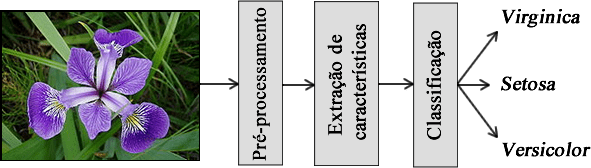
\includegraphics[scale=0.5]{img/irisExample.png}
{\fontsize{11pt}{\baselineskip}\selectfont
\\Fonte: \cite{pacheco2016agregaccao}
}
\end{figure}


\subsection{Redes Neurais Artificiais} %aqui falarei sobre redes neurais, somente introduzi grafos para pode explicar por completo ela
O ser humano possui capacidades cognitivas extraordinárias e, desde o surgimento da computação, desejou-se projetar máquinas capazes de realizar tarefas inteligentes que, até então, somente eram  executadas por humanos. Os primeiros trabalhos desenvolvidos nessa área foram: um neurônio apresentado por \cite{mcculloch1943logical}, usado posteriormente como base para a concepção do  \textit{Perceptron} por \cite{rosenblatt1958perceptron} e um neurônio chamado \textit{Adaline} por \cite{widrow1960adaptive}. Tais trabalhos deram origem ao conceito de RNA que, em outras palavras, é uma tentativa de copiar a estrutura e o funcionamento do cérebro, composto este por bilhões de neurônios, para uma estrutura artificial, transformando assim as redes neurais biológicas em redes neurais artificiais \citep{Rauber2005}.

Para compreender o conceito por trás de uma rede neural, é preciso introduzir um modelo simplificado de um neurônio e suas capacidades de processamento associadas. Cada neurônio é considerado como uma unidade básica de processamento que, quando estimulada por sinais de entrada, emitem sinais de saída como uma reação. Tais sinais emitidos por um neurônio, são repassados para outros neurônios através de uma conexão sináptica. Tal processo pode ser repetido por várias camadas de neurônios até chegar ao nosso cérebro, que então processa essa informação e produz novas reações \citep{baeza1999modern}. A principal função de uma rede neural é armazenar conhecimento experimental e torná-lo disponível, o que em prática significa que este conhecimento é adquirido e armazenado em pesos sinápticos durante o processo. Uma RNA é normalmente implementada através de um programa de computador (\textit{software}) ou através de componentes eletrônicos (\textit{hardware}).

 Uma rede neural pode ser representada matematicamente através de uma estrutura de grafo (Figura \ref{fig:graphNeuron}), em que os vértices fazem o papel dos neurônios e as arestas representam as conexões sinápticas entre os neurônios, no qual se adicionarmos pesos a tais arestas, é possível mensurar a força de tal conexão sináptica. Seja $x_i$ entradas fornecidas por outros neurônios para um neurônio artificial. O processamento desse neurônio consiste em uma combinação linear das $D$ entradas tais que $\sum_{i=1}^{D} = w_i x_i$, onde $x_i$ é uma aresta com peso $w_i$. Se tal valor ultrapassar um limiar $\mu$, esse neurônio dispara um valor positivo (1) na saída binária $y$, caso contrário dispara um valor negativo (0) na saída. 

\begin{figure}[ht!]
\caption{Diagrama de um neurônio artificial}
\label{fig:graphNeuron}
\centering
\includegraphics[scale=0.5]{img/graphNeuron.png}
{\fontsize{11pt}{\baselineskip}\selectfont
\\Fonte: \cite{Rauber2005}
}
\end{figure}

\subsection{\textit{K-vizinhos mais próximos}}
O algoritmo K-vizinhos mais próximos (do inglês: \textit{K-neareast neighbours} - KNN) tem como objetivo determinar o rótulo de classificação de uma amostra, baseando-se em outras amostras vizinhas, advindas de um conjunto de treinamento. O classificador KNN, um dois mais simples algoritmos de classificação, é baseado em
instâncias. Esse algoritmo encontra os $k$ objetos mais similares e realiza uma votação de acordo com as classes às quais pertencem esses $k$ objetos, assinalando por fim, uma classe ao objeto de teste. A literatura apresenta diversas formas para expressar essa distância/similaridade dentre os objetos de análise \citep{fukunaga1975knn, duda1973pattern}. Por exemplo, se os dados trabalhados estão em formato de texto, é comum utilizar a similaridade por cossenos. Por outro lado, se os dados possuírem formato numérico, possivelmente a distância euclidiana será mais eficaz.